\documentclass[border=1pt]{standalone}
% Shared preamble of the standalone figure sources (compiled to ../fig_*.pdf by build.sh).
\renewcommand{\rmdefault}{ptm}
\usepackage{amsmath,amssymb}
\usepackage[dvipsnames]{xcolor}
\usepackage{tikz}
\usetikzlibrary{arrows.meta,positioning,fit,calc,shapes.geometric,patterns,decorations.pathreplacing,backgrounds}
\usepackage{pgfplots}
\pgfplotsset{compat=1.17}
% ---------------------------------------------------------------------------
% Notation and helper macros (single source for symbols used in the paper)
% ---------------------------------------------------------------------------

% Placeholder for content that waits for the formal results or author input.
\newcommand{\todo}[1]{{\color{red}[\textbf{TODO:} #1]}}

% Generic
\newcommand{\R}{\mathbb{R}}
\newcommand{\SE}{\mathrm{SE}(3)}
\newcommand{\SO}{\mathrm{SO}(3)}
\newcommand{\T}{\top}
\newcommand{\E}{\mathbb{E}}
\newcommand{\norm}[1]{\left\lVert #1 \right\rVert}
\newcommand{\clip}{\operatorname{clip}}
\newcommand{\diag}{\operatorname{diag}}
\newcommand{\argmin}{\operatorname*{arg\,min}}
\newcommand{\lexmin}{\operatorname*{lex\,min}}

% Frames
\newcommand{\FI}{\mathcal{F}_{I}}
\newcommand{\FT}{\mathcal{F}_{T}}
\newcommand{\FC}{\mathcal{F}_{C}}
\newcommand{\FL}{\mathcal{F}_{L}}

% Mission
\newcommand{\Td}{T_{d}}            % mission deadline
\newcommand{\Dd}{\Delta_{d}}       % terminal reserve
\newcommand{\Lt}{L}                % latest admissible entry time
\newcommand{\Bmax}{B_{\max}}       % Delta-v budget
\newcommand{\dvused}{\Delta v_{\mathrm{u}}} % Delta-v used so far

% Geometry
\newcommand{\shat}{\hat{s}}
\newcommand{\er}{e_{r}}
\newcommand{\epol}{e_{\mathrm{pol}}}
\newcommand{\eaz}{e_{\mathrm{az}}}
\newcommand{\dlat}{\Delta\lambda}
\newcommand{\thg}{\theta_{g}}
\newcommand{\Tset}{\mathcal{T}}          % entry arrival-time candidates
\newcommand{\Wgeo}{\mathcal{W}_{\mathrm{geo}}}
\newcommand{\vb}{v_{b}}                  % braking envelope

% Decision and execution
\newcommand{\Bgrid}{\mathfrak{B}}        % candidate intent grid
\newcommand{\Bc}{\mathfrak{B}_{c}}       % certifiable candidate set
\newcommand{\Cmap}{\mathcal{C}}          % certification map
\newcommand{\zE}{z_{E}}                  % execution feedback
\newcommand{\PE}{P_{\mathcal{E}}}        % execution-layer macro kernel
\newcommand{\PC}{P_{\mathcal{C}}}        % certification-induced kernel
\newcommand{\gd}{\gamma_{d}}             % per-decision discount
\newcommand{\Hp}{H_{p}}                  % mode-prediction horizon
\newcommand{\ehat}{\hat{e}}
\newcommand{\tauhat}{\hat{\tau}}
\newcommand{\dvhat}{\widehat{\Delta v}}
\newcommand{\rtil}{\tilde{r}}

% Method names (fixed terminology, see fact sheet 00)
\newcommand{\ECC}{ECC}
\newcommand{\RWG}{RWG}

% Channel colors used in all method figures
\colorlet{actcol}{orange!85!black}   % action-level channel (screening)
\colorlet{actfill}{orange!14}
\colorlet{stcol}{blue!70!black}      % state-level channel (execution feedback)
\colorlet{stfill}{blue!7}
\colorlet{exefill}{green!8}
% Results figures: methods and outcomes, Okabe--Ito palette
\usepgfplotslibrary{fillbetween}
\definecolor{cECC}{HTML}{D55E00}    % ECC
\definecolor{cNOIN}{HTML}{E69F00}   % ECC w/o execution inputs (critic on the policy view)
\definecolor{cNOLE}{HTML}{0072B2}   % ECC w/o long-range entry (keep / correct only)
\definecolor{cNOCO}{HTML}{56B4E9}   % ECC w/o coordination
\definecolor{cSAC}{HTML}{555555}    % SAC--MPC
\definecolor{cTD3}{HTML}{000000}    % TD3--MPC
\definecolor{oCap}{HTML}{009E73}
\definecolor{oTime}{HTML}{BBBBBB}
\definecolor{oFuel}{HTML}{56B4E9}
\definecolor{oUns}{HTML}{CC79A7}
\pgfplotsset{resstyle/.style={tick label style={font=\scriptsize},label style={font=\footnotesize},
  legend style={font=\scriptsize,draw=none,fill=none},grid=major,grid style={gray!15},axis line style={gray!70!black}}}
% \band{group key}{color}{low column}{high column}: min--max band over seeds
\newcommand{\band}[4]{%
  \addplot[name path=lo#1#3,draw=none,forget plot] table[x=x,y=#3]{data/train_#1.dat};
  \addplot[name path=hi#1#3,draw=none,forget plot] table[x=x,y=#4]{data/train_#1.dat};
  \addplot[#2,fill opacity=0.15,forget plot] fill between[of=lo#1#3 and hi#1#3];}
% Case figures: execution modes (Table II)
\definecolor{cStage}{HTML}{0072B2}
\definecolor{cEntry}{HTML}{E69F00}
\definecolor{cHold}{HTML}{999999}
\definecolor{cDesc}{HTML}{009E73}
\colorlet{mStage}{cStage}\colorlet{mEntry}{cEntry}\colorlet{mHold}{cHold}\colorlet{mDesc}{cDesc}
% \modeband{t0}{t1}{mode style}: shaded mode interval over the full height of a time-history axis
\newcommand{\modeband}[3]{\fill[#3,opacity=0.13] ({axis cs:#1,1}|-{rel axis cs:0,0}) rectangle ({axis cs:#2,1}|-{rel axis cs:0,1});}

\begin{document}
% Sweep-cone geometry (single column), oblique projection
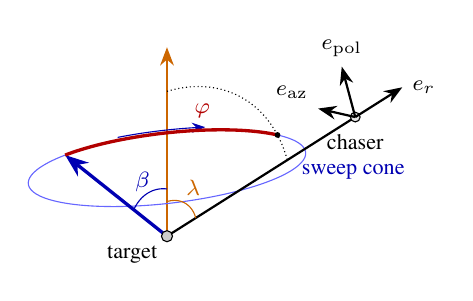
\begin{tikzpicture}[>=Stealth,font=\footnotesize,
  x={(1cm,0cm)},y={(-0.42cm,-0.30cm)},z={(0cm,1cm)},scale=0.80]
  \def\L{2.3}          % length of unit directions
  \def\bet{62}         % cone half-angle beta
  \def\lam{74}         % line-of-sight polar angle lambda
  \def\psip{200}       % azimuth of the port direction
  \def\psil{300}       % azimuth of the line of sight
  \def\D{3.6}          % chaser distance along the line of sight
  \pgfmathsetmacro{\R}{\L*sin(\bet)}
  \pgfmathsetmacro{\H}{\L*cos(\bet)}
  % spin axis
  \draw[->,thick,orange!80!black] (0,0,0) -- (0,0,3.0) node[anchor=south] {$\bs$};
  % sweep cone: base circle and two generators
  \draw[blue!60,thin] plot[domain=0:360,samples=90,smooth] ({\R*cos(\x)},{\R*sin(\x)},{\H});
  \node[blue!70!black,anchor=west] at ({1.02*\R*cos(5)},{1.02*\R*sin(5)},{\H}) {sweep cone};
  % rotation direction of the port
  \draw[->,blue!70!black] plot[domain=228:262,samples=20] ({1.08*\R*cos(\x)},{1.08*\R*sin(\x)},{\H});
  % port direction
  \draw[->,very thick,blue!70!black] (0,0,0) -- ({\R*cos(\psip)},{\R*sin(\psip)},{\H}) node[anchor=east] {$\bn$};
  % beta arc
  \draw[blue!70!black] plot[domain=0:\bet,samples=20] ({0.75*sin(\x)*cos(\psip)},{0.75*sin(\x)*sin(\psip)},{0.75*cos(\x)});
  \node[blue!70!black] at ({0.95*sin(\bet/2)*cos(\psip)},{0.95*sin(\bet/2)*sin(\psip)},{0.95*cos(\bet/2)}) {$\beta$};
  % phase arc on the cone circle from the port to the LOS meridian
  \draw[very thick,red!70!black] plot[domain=\psip:\psil,samples=40] ({\R*cos(\x)},{\R*sin(\x)},{\H});
  \node[red!70!black,anchor=south] at ({\R*cos(262)},{\R*sin(262)},{\H+0.04}) {$\varphi$};
  % meridian of the line of sight (dotted)
  \draw[densely dotted] plot[domain=0:\lam,samples=30] ({\L*sin(\x)*cos(\psil)},{\L*sin(\x)*sin(\psil)},{\L*cos(\x)});
  \fill ({\L*sin(\bet)*cos(\psil)},{\L*sin(\bet)*sin(\psil)},{\L*cos(\bet)}) circle (1.3pt);
  % line of sight to the chaser
  \pgfmathsetmacro{\cx}{\D*sin(\lam)*cos(\psil)}
  \pgfmathsetmacro{\cy}{\D*sin(\lam)*sin(\psil)}
  \pgfmathsetmacro{\cz}{\D*cos(\lam)}
  \draw[thick] (0,0,0) -- (\cx,\cy,\cz);
  \draw[orange!80!black] plot[domain=0:\lam,samples=20] ({0.55*sin(\x)*cos(\psil)},{0.55*sin(\x)*sin(\psil)},{0.55*cos(\x)});
  \node[orange!80!black] at ({0.8*sin(\lam/2)*cos(\psil)},{0.8*sin(\lam/2)*sin(\psil)},{0.8*cos(\lam/2)}) {$\lambda$};
  % local basis at the chaser
  \pgfmathsetmacro{\erx}{sin(\lam)*cos(\psil)}  \pgfmathsetmacro{\ery}{sin(\lam)*sin(\psil)}  \pgfmathsetmacro{\erz}{cos(\lam)}
  \pgfmathsetmacro{\epx}{-cos(\lam)*cos(\psil)} \pgfmathsetmacro{\epy}{-cos(\lam)*sin(\psil)} \pgfmathsetmacro{\epz}{sin(\lam)}
  \pgfmathsetmacro{\eax}{sin(\psil)}            \pgfmathsetmacro{\eay}{-cos(\psil)}
  \filldraw[fill=gray!20] (\cx,\cy,\cz) circle (2.2pt);
  \node[anchor=north] at (\cx,\cy,\cz-0.12) {chaser};
  \draw[->,thick] (\cx,\cy,\cz) -- ++(0.9*\erx,0.9*\ery,0.9*\erz) node[anchor=west] {$\er$};
  \draw[->,thick] (\cx,\cy,\cz) -- ++(0.9*\epx,0.9*\epy,0.9*\epz) node[anchor=south] {$\epol$};
  \draw[->,thick] (\cx,\cy,\cz) -- ++(0.9*\eax,0.9*\eay,0) node[anchor=south east] {$\eaz$};
  % target
  \filldraw[fill=gray!40] (0,0,0) circle (2.5pt);
  \node[anchor=north east] at (0,0,0) {target};
\end{tikzpicture}
\end{document}
